\title{第七周作业}
\author{洪艺中}
\maketitle
\section{第一次作业}
\subsection*{89页 题目2}
\begin{problem*}
设矩阵 $\ma \in \field^{m \times n}$, $\mb \in \field$, 证明 $r(\me_m - \ma\mb) + n = r(\me_n - \mb\ma) + m$.
\end{problem*}
\begin{solution}
构造
\[
\mm := \begin{pmatrix}
    \me_m & \ma \\
    \mb & \me_n
\end{pmatrix},
\]
利用分块矩阵的初等变换, 可以得到
\[
\begin{aligned}
    r(\me_m - \ma\mb) + n
    =&
    r\left(\begin{pmatrix}
        \me_m - \ma\mb &  \\
         & \me_n
    \end{pmatrix}\right) \\
    =&
    r\left(\begin{pmatrix}
        \me_m & \ma \\
        \mb & \me_n
    \end{pmatrix}\right) \\
    =& r\left(\begin{pmatrix}
        \me_m &  \\
         & \me_n - \mb\ma
    \end{pmatrix}\right)
    =
    r(\me_n - \mb\ma) + m,
\end{aligned}
\]
所以命题得证.
\end{solution}

\subsection*{题目3}
\begin{problem*}
设 $\ma$ 是 $m \times n$ 矩阵, $\mb$ 是 $n \times m$ 矩阵, 且 $n \geqslant m$. 若 $\ma \mb = \me_m$, 证明 $r(\ma) = m = r(\mb)$.
\end{problem*}
\begin{solution}
因为 $ n \geqslant m$, 并且矩阵的秩不超过其行列规模的较小值. 所以 $r(\ma) \leqslant m$, $r(\mb) \leqslant m$. 利用乘积秩的不等式
\[
    m = r(\ma \mb) \leqslant \min\{r(\ma), r(\mb)\} \leqslant m,
\]
所以上面的 $\leqslant $ 必须取到相等. 因此 $r(\ma) = r(\mb) = m$. 命题得证.
\end{solution}

\newpage
\subsection*{题目4}
\begin{problem*}
设 $\ma$ 为 $n$ 阶矩阵 ($n \geqslant 2$),  $\ma^{\ast}$ 为 $\ma$ 的伴随阵. 证明
\[
r(\ma^{\ast}) = 
\begin{cases}
    n, & r(\ma) = n, \\
    1, & r(\ma) = n - 1, \\
    0, & r(\ma) \leqslant n - 2.
\end{cases}
\]
\end{problem*}
\begin{solution}
\begin{enumerate}
    \item $r(\ma) = n$ 时, $\ma$ 可逆, 所以 $\ma^{\ast}$ 也可逆. 因此 $r(\ma^{\ast}) = n$;
    \item $r(\ma) = n - 1$ 时, 借助 Sylvester 不等式,
    \[
        r(\ma \ma^{\ast}) \geqslant r(\ma) + r(\ma^\ast) - n,
    \]
    因为 $|\ma| = 0$, 所以 $\ma \ma^{\ast} = \mo$. 因此代入 $r(\ma \ma^{\ast}) = 0$, $r(\ma) = n - 1$ 得到
    \[
        0 \geqslant n - 1 + r(\ma^\ast) - n = r(\ma^\ast) - 1,
    \]
    所以 $r(\ma^\ast) \leqslant 1$. 同时, 因为 $r(\ma) = n - 1$, 所以 $\ma$ 中有非零的 $n - 1$ 阶子式. 因此 $\ma^\ast$ 中有非零元素. 所以 $r(\ma^\ast) > 0$. 因此有 $0 < r(\ma^\ast) \leqslant 1$, 所以 $r(\ma^\ast) = 1$.
    \item $r(\ma) \leqslant n - 2$ 时, $\ma$ 的所有 $n - 1$ 阶子式都是 $0$. 故 $\ma^\ast = \mo$, 所以 $r(\ma^\ast) = 0$.
\end{enumerate}
\end{solution}

\subsection*{ 题目 7 }
\begin{problem*}
证明: 若 $\ma$, $\mb$ 是 $n$ 阶方阵, 且 $\ma \mb = \mo$, 那么 $r(\ma) + r(\mb) \leqslant n$.
\end{problem*}
\begin{solution}
用 Sylvester 不等式立即可得.
\end{solution}

\newpage
\subsection*{ 100页 题目2 (1) }
\begin{problem*}
    用作图法证明 $(\mla + \mlb) + (\mla - \mlb) = 2\mla$.
\end{problem*}
\begin{solution}
    \begin{figure}[htb]
        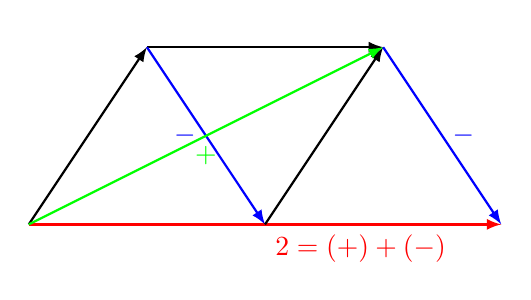
\begin{tikzpicture}[scale=1.5, >=latex]
            \draw[->, thick, red, ] (0, 0) -- (4, 0) node[midway, below right] {$2\mla = (\mla + \mlb) + (\mla - \mlb)$};
            
            \draw[->, thick] (1, 1.5) -- ++(2, 0) node[midway, above] {$\mla$} coordinate (A);
            \draw[->, thick] (0, 0) -- (1, 1.5) node[midway, above left] {$\mlb$} coordinate (B);
            \draw[->, thick, blue] (B) -- (2, 0) node[midway, left] {$\mla - \mlb$} ;
            
            \draw[->, thick] (2, 0) -- ++(1, 1.5) node[midway, above left] {$\mlb$} coordinate (D);
            \draw[->, thick, green] (0, 0) -- (D) node[midway, below] {$\mla + \mlb$} ;
            
            \draw[->, thick, blue] (D) -- ++(1, -1.5) node[midway, right] {$\mla - \mlb$};
        \end{tikzpicture}
    \end{figure}
\end{solution}

\subsection*{ 题目 3 偶数 }
\begin{problem*}
    向量 $\mla$, $\mlb$ 需要满足什么条件, 以下各式才成立?
\begin{enumerate}
    \item[(2)] $\mla + \mlb = \lambda(\mla + \mlb)$;
    \item[(4)] $|\mla + \mlb| = |\mla| + |\mlb|$;
    \item[(6)] $|\mla - \mlb| = |\mla| - |\mlb|$;
\end{enumerate}
\end{problem*}
\begin{solution}
\begin{enumerate}
    \item[(2)] 移项得到 $(\lambda - 1)\mla = (\lambda + 1)\mlb$. 所以 $\lambda \not= 1$ 时, $\mla = (\lambda + 1)\mlb / (\lambda - 1)$, $\lambda = 1$ 时, $\mlb = 0$ 即可;
    \item[(4)] 存在 $k, l \in \real$, $k\mla = l\mlb$ 且 $kl \geqslant 0$;
    \item[(6)] 存在 $k, l \in \real$, $k\mla = l\mlb$ 且 $kl \leqslant 0$.
\end{enumerate}
\end{solution}

\subsection*{ 题目 4 }
\begin{problem*}
用向量法证明任意三角形两边中点的连线平行于第三边, 而且它的长等于第三边长的一半.
\end{problem*}
\begin{solution}
设三角形为 $ABC$ 如下图.
\begin{figure}[htb]
    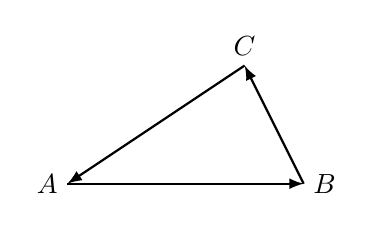
\begin{tikzpicture}[scale=1.5, >=latex]
        \draw (0, 0) node[left] {$A$} coordinate (A);
        \draw (2, 0) node[right] {$B$} coordinate (B);
        \draw (1.5, 1) node[above] {$C$} coordinate (C);
        \draw[->, thick] (A) -- (B) node[midway, below] {$\mlc$};
        \draw[->, thick] (B) -- (C) node[midway, above right] {$\mla$};
        \draw[->, thick] (C) -- (A) node[midway, above left] {$\mlb$};
    \end{tikzpicture}
\end{figure}
对于这个问题, 不妨选择 $CA$, $BC$ 两边, 若非如此, 只需要变换字母标记即可. 这两条边中点的连线为 $(\mla + \mlb) / 2$. 第三边 $\mlc = -\mlb - \mla$, 二者成倍数, 所以平行. 中线的长度是 $|(\mla + \mlb) / 2| = |-\mlc / 2| = |\mlc| / 2$, 所以长度是第三边的一半.
\end{solution}

\newcommand{\lvec}[1]{\overrightarrow{#1}}

\subsection*{ 题目 5 }
\begin{problem*}
设 $P$ 是平行四边形 $ABCD$ 的中心, $O$ 是任意一点. 证明 $\lvec{OA} + \lvec{OB} + \lvec{OC} + \lvec{OD} = 4\lvec{OP}$.
\end{problem*}
\begin{solution}
首先, 平行四边形的中心是其两个对角线的交点. 根据平面几何的知识, 中点关于 $A$ 的方位向量是 $\lvec{AP} = \frac{1}{2}\lvec{AC}$. 因此
\[
\begin{aligned}
     {} & \lvec{OA} + \lvec{OB} + \lvec{OC} + \lvec{OD} \\
    ={} & 4\lvec{OA} + (\lvec{AB} + \lvec{AC} + \lvec{AD}) \\
    ={} & 4\lvec{OA} + 2\lvec{AC} \\
    ={} & 4\lvec{OA} + 4\lvec{AP} = 4\lvec{OP}.
\end{aligned}
\]
\end{solution}

\subsection*{ 题目 6 }
\begin{problem*}
设 $O$ 是平面上多边形 $A_1 A_2 \cdots A_n$ 的中心, 证明 $\lvec{OA_1} + \lvec{OA_2} + \cdots + \lvec{OA_n} = 0$.
\end{problem*}
\begin{solution}
因为正多边形绕 $O$ 旋转 $2 \pi / n$ 后与原来重合, 所以旋转前后 $\lvec{OA_1} + \lvec{OA_2} + \cdots + \lvec{OA_n}$ 是不变的. 如果一个向量旋转 $\alpha$($0 < \alpha < \pi$) 之后和自己相等, 说明它只能是 $\mat{0}$. (否则一个向量旋转 $\alpha$ 之后与自己不共线, 但是相等又说明共线, 产生矛盾) 因此   $\lvec{OA_1} + \lvec{OA_2} + \cdots + \lvec{OA_n} = 0$.
\end{solution}

\subsection*{ 题目 8 }
\begin{problem*}
已知 $\lvec{OA} = \mlr_1$, $\lvec{OB} = \mlr_2$, $\lvec{OC} = \mlr_3$ 是以原点 $O$ 为顶点的平行六面体的三条边, 设过点 $O$ 的对角线与平面 $ABC$ 的交点为 $M$, 求向量 $\lvec{OM}$.
\end{problem*}
\begin{solution}
    \begin{figure}[htbp]
        \centering
        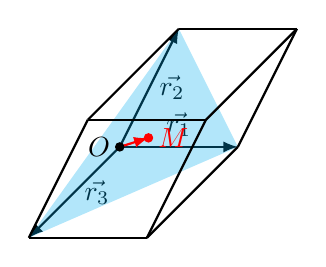
\begin{tikzpicture}[scale=1.5, >=latex]
            % 定义参数
            \pgfmathsetmacro{\ax}{1} % A 的 x 坐标
            \pgfmathsetmacro{\ay}{0} % A 的 y 坐标
            \pgfmathsetmacro{\az}{0} % A 的 z 坐标
        
            \pgfmathsetmacro{\bx}{0.5} % B 的 x 坐标
            \pgfmathsetmacro{\by}{1} % B 的 y 坐标
            \pgfmathsetmacro{\bz}{0} % B 的 z 坐标
        
            \pgfmathsetmacro{\cx}{0} % C 的 x 坐标
            \pgfmathsetmacro{\cy}{0} % C 的 y 坐标
            \pgfmathsetmacro{\cz}{2} % C 的 z 坐标
        
            % 定义点 O
            \coordinate (O) at (0, 0, 0);
            
            % 定义点 A, B, C
            \coordinate (A) at (\ax, \ay, \az);
            \coordinate (B) at (\bx, \by, \bz);
            \coordinate (C) at (\cx, \cy, \cz);
            
            % 绘制向量 OA, OB, OC
            \draw[->, thick] (O) -- (A) node[midway, above] {$\vec{r_1}$};
            \draw[->, thick] (O) -- (B) node[midway, right] {$\vec{r_2}$};
            \draw[->, thick] (O) -- (C) node[midway, right] {$\vec{r_3}$};
            
            % 计算其他点 D, E, F, G
            \coordinate (D) at (\ax + \bx, \ay + \by, \az + \bz); % A + B
            \coordinate (E) at (\ax + \cx, \ay + \cy, \az + \cz); % A + C
            \coordinate (F) at (\bx + \cx, \by + \cy, \bz + \cz); % B + C
            \coordinate (G) at (\ax + \bx + \cx, \ay + \by + \cy, \az + \bz + \cz); % A + B + C
            \pgfmathsetmacro{\mx}{(\ax + \bx + \cx) / 3}
            \pgfmathsetmacro{\my}{(\ay + \by + \cy) / 3}
            \pgfmathsetmacro{\mz}{(\az + \bz + \cz) / 3}
            \coordinate (M) at (\mx, \my, \mz);
        
            \fill[cyan, opacity=0.3] (A) -- (B) -- (C) -- cycle;

            % 绘制平行六面体的其他边
            \draw[thick] (A) -- (D);
            \draw[thick] (A) -- (E);
            \draw[thick] (B) -- (D);
            \draw[thick] (B) -- (F);
            \draw[thick] (C) -- (E);
            \draw[thick] (C) -- (F);
            \draw[thick] (D) -- (G);
            \draw[thick] (E) -- (G);
            \draw[thick] (F) -- (G);
        
            % 绘制 OM
            \draw[->, thick, red] (O) -- (M);
        
            % 绘制点 O 和 M
            \filldraw[black] (O) circle (1pt) node[left] {$O$};
            \filldraw[red] (M) circle (1pt) node[right] {$M$};
        \end{tikzpicture}
    \end{figure}
    点 $M$ 在平面 $ABC$ 上, 就是说 $\lvec{AM}$ 可以用 $\lvec{AB}$ 和 $\lvec{AC}$ 线性表示. 所以设 $\lvec{OM} = k(\mlr_1 + \mlr_2 + \mlr_3)$, 就存在 $a, b \in \real$,
    \[
        \lvec{AM} = a\lvec{AB} + b\lvec{AC},
    \]
    即
    \[
        k(\mlr_1 + \mlr_2 + \mlr_3) - \mlr_1 = a(\mlr_2 - \mlr_1) + b(\mlr_3 - \mlr_1),
    \]
    合并同类项, 得到
    \[
        (k - 1 + a + b)\mlr_1 + (k - a)\mlr_2 + (k - b)\mlr_3 = \mat{0}.
    \]
    由于 $\mlr_1, \mlr_2, \mlr_3$ 线性无关, 所以三个系数都必须是 $0$. 因此 $k = a = b = \dfrac{1}{3}$. 即
    \[
    \lvec{OM} = \dfrac{1}{3}(\mlr_1 + \mlr_2 + \mlr_3).
    \]
\end{solution}

\newpage
\section{第二次作业}
\subsection*{ 问题 11 }
\begin{problem*}
在四面体 $OABC$ 中, 设点 $P$ 是 $\triangle ABC$ 的重心. 求向量 $\lvec{OP}$ 关于向量 $\lvec{OA}$, $\lvec{OB}$, $\lvec{OC}$ 的分解式.
\end{problem*}
\begin{solution}
    \begin{figure}[h]
        \centering
        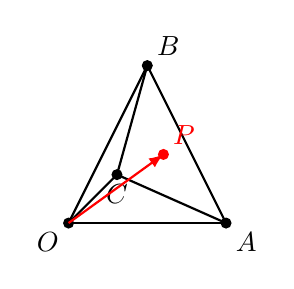
\begin{tikzpicture}[>=latex]
            % 定义点
            \coordinate (O) at (0, 0, 0);
            \coordinate (A) at (2, 0, 0);
            \coordinate (B) at (1, 2, 0);
            \coordinate (C) at (1, 1, 1);
            \coordinate (P) at (4/3, 1, 1/3); % 重心 P
    
            % 绘制四面体的边
            \draw[thick] (O) -- (A);
            \draw[thick] (O) -- (B);
            \draw[thick] (O) -- (C);
            \draw[thick] (A) -- (B);
            \draw[thick] (A) -- (C);
            \draw[thick] (B) -- (C);
    
            % 绘制重心 P
            \fill[red] (P) circle (2pt) node[above right] {$P$};
    
            % 标记点
            \fill[] (O) circle (2pt) node[below left] {$O$};
            \fill[] (A) circle (2pt) node[below right] {$A$};
            \fill[] (B) circle (2pt) node[above right] {$B$};
            \fill[] (C) circle (2pt) node[below] {$C$};

            \draw[->, thick, red] (O) -- (P);
        \end{tikzpicture}
    \end{figure}
    利用例 4.1.5 的结论, 中心到顶点的距离相当于这个顶点所引中线长的 $\dfrac{2}{3}$. 所以
    \[
    \begin{aligned}
        \lvec{OP} 
        ={}& \lvec{OA} + \lvec{AP} \\
        ={}& \lvec{OA} + \frac{2}{3} \times \frac{1}{2}(\lvec{AB} + \lvec{AC}) \\
        ={}& \lvec{OA} + \frac{1}{3}(\lvec{OB} - \lvec{OA} + \lvec{OC} - \lvec{OA}) \\
        ={}& \frac{1}{3}(\lvec{OA} + \lvec{OB} + \lvec{OC})
    \end{aligned}
    \]
\end{solution}

\subsection*{ 题目 15 }
\begin{problem*}
证明三个向量 $a\mle_1 - b\mle_2$, $b\mle_2 - c\mle_3$, $c\mle_3 - a\mle_1$ 共面.
\end{problem*}
\begin{solution}
因为 $(a\mle_1 - b\mle_2) + (b\mle_2 - c\mle_3) + (c\mle_3 - a\mle_1) = \mat{0}$, 所以三个向量线性相关. 根据推论 4.1.8, 三个向量共面.
\end{solution}

\newpage
\subsection*{ 106 页 题目 1 }
\begin{problem*}
    在平行六面体 \( ABCD - EFGH \) 中, 平行四边形 $CGHD$ 的中心为 $P$, 并设 \( \lvec{EF} = \mle_1 \), \( \lvec{EH} = \mle_2 \), \( \lvec{EA} = \mle_3 \). 试求向量 $\lvec{AP}$, $\lvec{FP}$ 关于标架 $\{A; \mle_1, \mle_2, \mle_3\}$, 以及 \( \triangle BEP \) 三个顶点及其重心关于 $\{A; \mle_1, \mle_2, \mle_3\}$ 的坐标.
\end{problem*}
\begin{solution}
    \begin{figure}[htb]
        \centering
        \begin{tikzpicture}[scale=2, >=latex]
    
            % Define coordinates for points
            \coordinate (A) at (0, 0, 0);
            \coordinate (B) at (2, 0, 0);
            \coordinate (D) at (0.5, 1, 0);
            \coordinate (C) at (2.5, 1, 0);
            \coordinate (E) at (0, 0, 1.5);
            \coordinate (F) at (2, 0, 1.5);
            \coordinate (H) at (0.5, 1, 1.5);
            \coordinate (G) at (2.5, 1, 1.5);
            \coordinate (I) at ($1/2*(B) + 1/3*(D) + 1/2*(E)$);
    
            % Define center of parallelogram CGHD as point P
            \coordinate (P) at ($0.5*(C) + 0.5*(H)$);
    
            % Draw edges of the parallelepiped
            \draw[thick] (A) -- (B) -- (C) -- (D) -- cycle;
            \draw[thick] (E) -- (F) -- (G) -- (H) -- cycle;
            \draw[thick] (A) -- (E);
            \draw[thick] (B) -- (F);
            \draw[thick] (C) -- (G);
            \draw[thick] (D) -- (H);
    
            % Highlight parallelogram CGHD
            \fill[blue!10, opacity=0.5] (C) -- (G) -- (H) -- (D) -- cycle;
    
            % Draw vectors EF, EH, EA with arrows and labels
            \draw[->, thick, blue] (E) -- (F) node[midway, below right] {$\mathbf{e}_1$};
            \draw[->, thick, blue] (E) -- (H) node[midway, left] {$\mathbf{e}_2$};
            \draw[->, thick, blue] (E) -- (A) node[midway, right] {$\mathbf{e}_3$};
    
            % Draw vectors AP and FP
            \draw[->, thick, purple] (A) -- (P) ;
            \draw[->, thick, purple] (F) -- (P) ;
    
            % Draw triangle BEP and its centroid
            \draw[thick, green] (B) -- (E) -- (P) -- cycle;
            \fill[green] (I) circle (2pt) node[below] {centoid};
            % \fill[] circle (2pt) at ($ (B)!0.33!(E)!0.33!(P) $)  [below] {centoid};
    
            % Label points
            \node[left] at (A) {$A$};
            \node[below right] at (B) {$B$};
            \node[below right] at (C) {$C$};
            \node[left] at (D) {$D$};
            \node[left] at (E) {$E$};
            \node[right] at (F) {$F$};
            \node[right] at (G) {$G$};
            \node[left] at (H) {$H$};
            \node[left] at (P) {$P$};
    
        \end{tikzpicture}
    \end{figure}

    用前面的题目 5, $\lvec{EP} = \frac{1}{4}(\lvec{EH} + \lvec{EG} + \lvec{EC} + \lvec{ED})$. 因此
    \[
        \lvec{EP} = \frac{1}{4}(\mle_2 + (\mle_1 + \mle_2) + (\mle_1 + \mle_2 + \mle_3) + (\mle_2 + \mle_3)) = \frac{1}{2}\mle_1 + \mle_2 + \frac{1}{2}\mle_3,
    \]
    所以 $\lvec{AP} = \frac{1}{2}\mle_1 + \mle_2 - \frac{1}{2}\mle_3 = (\frac{1}{2}, 1, -\frac{1}{2})$, $\lvec{FP} = -\frac{1}{2}\mle_1 + \mle_2 + \frac{1}{2}\mle_3 = (-\frac{1}{2}, 1, \frac{1}{2})$.

    $B$ 的坐标由 $\lvec{AB}$ 决定, 为 $(1, 0, 0)$, 同理可以写出 $E = (0, 0, -1)$, $P = (\frac{1}{2}, 1, -\frac{1}{2})$. 因此 $\triangle BEP$ 的重心是 $(\frac{1}{2}, \frac{1}{3}, -\frac{1}{2})$.
\end{solution}